\iffalse
\title{PH:2018}
\author{AI24BTECH11007}
\section{ph}
\chapter{2018}
\fi

                       
    \item An interstellar object has speed $v$ at the point of its shortest distance $R$ from a star of much larger mass $M$. Given $v^2 = \frac{2GM}{R}$, the trajectory of the object is:

    \hfill{(PH:2018)}
		\begin{multicols}{4}
    \begin{enumerate}
        \item circle
        \item ellipse
        \item parabola
        \item hyperbola
    \end{enumerate}
		\end{multicols}
   

    \item A particle moves in one dimension under a potential $V(x) = \alpha |x|$ with some non-zero total energy. Which one of the following best describes the particle trajectory in the phase space?

    \hfill{(PH:2018)}
		\begin{multicols}{2}
    \begin{enumerate}
	    \item 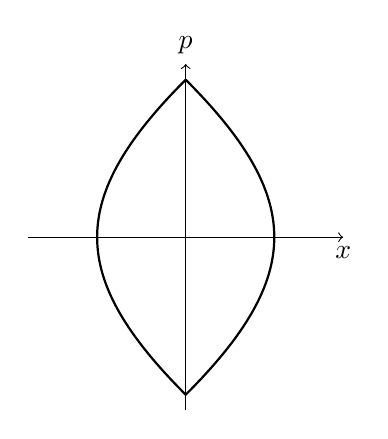
\begin{tikzpicture}
    % Draw the axes
    \draw[->] (-2, 0) -- (2, 0) node[below] {$x$};
    \draw[->] (0, -2.2) -- (0, 2.2) node[above] {$p$};
    
    % Draw the shape using Bézier curves
    \draw[thick] (0, 2) .. controls (1.5, 0.5) and (1.5, -0.5) .. (0, -2)
                 .. controls (-1.5, -0.5) and (-1.5, 0.5) .. (0, 2);
\end{tikzpicture}

        \item 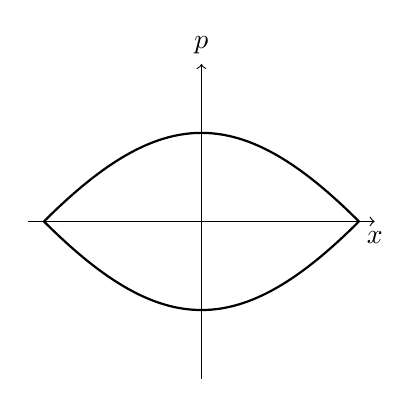
\begin{tikzpicture}
    % Draw the axes
    \draw[->] (-2.2, 0) -- (2.2, 0) node[below] {$x$};
    \draw[->] (0, -2) -- (0, 2) node[above] {$p$};
    
    % Draw the shape using Bézier curves
    \draw[thick] (2,0) .. controls (0.5, 1.5) and (-0.5, 1.5) .. (-2, 0)
                 .. controls (-0.5, -1.5) and (0.5, -1.5) .. (2, 0);
\end{tikzpicture}


        \item 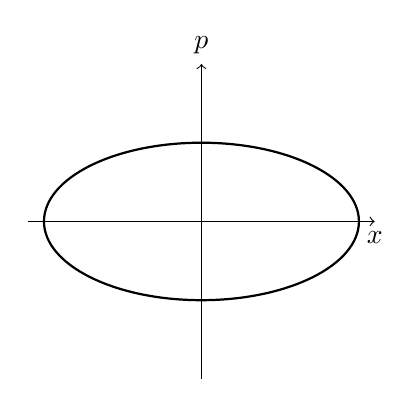
\begin{tikzpicture}
    % Draw the axes
    \draw[->] (-2.2, 0) -- (2.2, 0) node[below] {$x$};
    \draw[->] (0, -2) -- (0, 2) node[above] {$p$};
    
    % Draw the ellipse
    \draw[thick] (0, 0) ellipse (2 and 1);
\end{tikzpicture}

        \item \begin{tikzpicture}
    % Draw the rectangle
    \draw (-2, -1) rectangle (2, 1);
    
    % Draw the axes
    \draw[->] (-2.2, 0) -- (2.2, 0) node[right] {$x$};
    \draw[->] (0, -2) -- (0, 2) node[above] {$p$};
\end{tikzpicture}

    \end{enumerate}
			\end{multicols}
    

    \item Consider an infinitely long solenoid with $N$ turns per unit length, radius $R$ and carrying a current $I(t) = \alpha \cos \omega t$, where $\alpha$ is a constant and $\omega$ is the angular frequency. The magnitude of the electric field at the surface of the solenoid is:

    \hfill{(PH:2018)}
		\begin{multicols}{2}
    \begin{enumerate}
        \item $\frac{1}{2} \mu_0 N R \omega \alpha \sin \omega t$
        \item $\frac{1}{2} \mu_0 \omega N R \cos \omega t$
        \item $\mu_0 N R \omega \alpha \sin \omega t$
        \item $\mu_0 \omega N R \cos \omega t$
    \end{enumerate}
\end{multicols}

    \item A constant and uniform magnetic field $\vec{B} = B_0 \hat{z}$ pervades all space. Which one of the following is the correct choice for the vector potential in Coulomb gauge?

    \hfill{(PH:2018)}
		\begin{multicols}{4}
    \begin{enumerate}
        \item $-B_0(x + y)\hat{i}$
        \item $B_0(x + y)\hat{j}$
        \item $B_0 x \hat{j}$
        \item $-\frac{1}{2} B_0 (x\hat{i} - y\hat{j})$
    \end{enumerate}
			\end{multicols}
    

    \item If $H$ is the Hamiltonian for a free particle with mass $m$, the commutator $[x, [x, H]]$ is:

    \hfill{(PH:2018)}
		\begin{multicols}{4}
    \begin{enumerate}
        \item $\frac{\hbar^2}{m}$
        \item $-\frac{\hbar^2}{m}$
        \item $-\frac{\hbar^2}{2m}$
        \item $\frac{\hbar^2}{2m}$
    \end{enumerate}
			\end{multicols}
 

    \item A long straight wire, having radius $a$ and resistance per unit length $r$, carries a current $I$. The magnitude and direction of the Poynting vector on the surface of the wire is:

    \hfill{(PH:2018)}
    \begin{enumerate}
        \item $\frac{I^2 r}{2\pi a}$, perpendicular to the axis of the wire and pointing inwards
        \item $\frac{I^2 r}{2\pi a}$, perpendicular to the axis of the wire and pointing outwards
        \item $\frac{I^2 r}{\pi a}$, perpendicular to the axis of the wire and pointing inwards
        \item $\frac{I^2 r}{\pi a}$, perpendicular to the axis of the wire and pointing outwards
    \end{enumerate}
   

    \item Three particles are to be distributed in four non-degenerate energy levels. The possible number of ways of distribution: (i) for distinguishable particles, and (ii) for identical Bosons, respectively, is:

    \hfill{(PH:2018)}
    \begin{multicols}{4}
    \begin{enumerate}
        \item (i) $24$, (ii) $4$
        \item (i) $24$, (ii) $20$
        \item (i) $64$, (ii) $20$
        \item (i) $64$, (ii) $16$
    \end{enumerate}
	    \end{multicols}
  

    \item The term symbol for the electronic ground state of oxygen atom is:

    \hfill{(PH:2018)}
    \begin{multicols}{4}
    \begin{enumerate}
        \item $^1S_0$
        \item $^1D_{2}$
        \item $^3P_0$
        \item $^3P_{2}$
    \end{enumerate}
	    \end{multicols}
    

    \item The energy dispersion for electrons in one dimensional lattice with lattice parameter $a$ is given by $E(k) = E_0 - \frac{1}{2}W \cos ka$, where $W$ and $E_0$ are constants. The effective mass of the electron near the bottom of the band is:

    \hfill{(PH:2018)}
    \begin{multicols}{4}
    \begin{enumerate}
        \item $\frac{2\hbar^2}{W a^2}$
        \item $\frac{\hbar^2}{W a^2}$
        \item $\frac{\hbar^2}{2W a^2}$
        \item $\frac{\hbar^2}{4W a^2}$
    \end{enumerate}
	    \end{multicols}


    \item Amongst electrical resistivity ($\rho$), thermal conductivity ($\kappa$), specific heat ($C$), Young's modulus ($Y$), and magnetic susceptibility ($\chi$), which quantities show a sharp change at the superconducting transition temperature?

    \hfill{(PH:2018)}
    \begin{multicols}{4}
    \begin{enumerate}
        \item $\rho, \kappa, C, Y$
        \item $\rho, C, \chi$
        \item $\rho, \kappa, C, \chi$
        \item $\kappa, Y, \chi$
    \end{enumerate}
	    \end{multicols}
  
  \item	  A quarter wave plate introduces a path difference of $\frac{\lambda}{4}$ between the two components of polarization parallel and perpendicular to the optic axis. An electromagnetic wave with $\overrightarrow{E} = (\hat{x} + \hat{y}) E_0 e^{i(kz - \omega t)} $ is incident normally on a quarter wave plate which has its optic axis making an angle $135\deg$ with the $x$-axis as shown.\\
	  \begin{center}
		  \begin{tikzpicture}
    % Draw the x and y axes
    \draw[->] (-1.5, 0) -- (1.5, 0) node[right] {$x$};
    \draw[->] (0, -1.5) -- (0, 1.5) node[above] {$y$};
    
    % Draw the optic axis at 135° angle
    \draw[dashed, ->] (1.2, -1.2) -- (-1.2, 1.2);
    \node at (-2, 1) {Optic axis};

    
    % Draw the 135° angle arc
    \draw[->] (0.5, 0) arc[start angle=0, end angle=135, radius=0.5];
    \node at (0.8, 0.3) {$135^\circ$};
\end{tikzpicture}


	  \end{center}
	  The emergent electromagnetic wave would be

	  \hfill{(PH:2018)}
	  \begin{enumerate}
		  \item elliptically polarized
		  \item circularly polarized
		  \item linearly polarized with polarization as that of incident wave
		  \item linearly polarized but with polarization at $90\deg$ to that of the incident wave
	  \end{enumerate}
  \item
	  A $p$-doped semiconductor slab carries a current $I=100mA$ in a magnetic field $B=0.2T$ as shown. One measures $V_y =0.25mV$ and $V_x =2mV$. The mobility of holes in the semiconductor is \rule{2cm}{0.4pt}$m^2 V^{-1} s^{-1}$(up to two decimal places).

	  \hfill{(PH:2018)}
	  \begin{center}
		  
\begin{circuitikz}
\tikzstyle{every node}=[font=\large]
\draw  (5.25,12.75) -- (11.25,12.75) -- (12.75,14.75) -- (6.75,14.75) -- cycle;
\draw  (5.25,12.25) rectangle (11.25,12.75);
\draw [short] (12.75,14.75) -- (12.75,14.25);
\draw [short] (11.25,12.25) -- (12.75,14.25);
\draw [<->, >=Stealth] (5.25,12) -- (11,12);
\node [font=\small] at (7.75,11.75) {l = 10 mm};
\draw [<->, >=Stealth] (11.5,12.25) -- (12.75,14);
\node [font=\small, rotate around={-307:(0,0)}] at (12.5,13) {w = 4 mm};
\node [font=\LARGE] at (8,15.25) {B};
\draw [->, >=Stealth] (8.5,15.5) -- (8.5,15);
\node [font=\LARGE] at (7,13.75) {I};
\draw [->, >=Stealth] (7.25,13.75) -- (7.75,13.75);
\draw [->, >=Stealth] (10.75,16.5) -- (12,16.5);
\draw [->, >=Stealth] (10.75,16.5) -- (10.75,15.5);
\draw [->, >=Stealth] (10.75,16.5) -- (10,15.75);
\node [font=\small] at (12.25,16.5) {x};
\node [font=\small] at (9.75,15.75) {y};
\node [font=\small] at (11,15.5) {z};
\draw [<->, >=Stealth] (13,14.75) -- (13,14.25);
\node [font=\small] at (13.75,14.5) {t = 1 mm};
\draw [short] (5.25,12.75) .. controls (4.75,11.5) and (3.75,10.75) .. (6.75,10.25);
\node [font=\large] at (7.25,10.25) {$V_x$};
\draw  (7.25,10.25) circle (0.5cm);
\draw [short] (7.75,10.25) .. controls (11.25,10) and (12,10.5) .. (11.25,12.75);
\node [font=\large] at (4.75,14.25) {$V_y$};
\draw  (4.75,14.25) circle (0.5cm);
\draw [short] (5,14.75) .. controls (5.75,15.25) and (6,15) .. (6.75,14.75);
\draw [short] (4.25,14) .. controls (3.75,13.5) and (4,12.75) .. (5.25,12.75);
\end{circuitikz}



	  \end{center}

  \item
	  An n-channel FET having Gate-Source switch-off voltage $V_{GS(OFF)}=-2V$ is used to invert a $0-5V$ square-wave signal as shown. The maximum allowed value of $R$ would be \rule{2cm}{0.4pt}$k\ohm$ (up to two decimal places).

	  \hfill{(PH:2018)}
 \begin{center}
		  
\begin{circuitikz}
\tikzstyle{every node}=[font=\normalsize]
\node at (10.5,14.75) [circ] {};
\draw [->, >=Stealth] (10.5,14.75) -- (11.75,14.75);
\draw (10.5,14.75) to[R] (10.5,12.5);
\draw (10.5,14.75) to[R] (8.25,14.75);
\draw (8.5,14.75) to[short, -o] (8.25,14.75) ;
\draw (11.75,15.5) to[short] (11.75,14.5);
\draw (11.75,14.75) to[short] (12.25,14.75);
\draw (11.75,15.25) to[short] (12.25,15.25);
\draw (12.25,14.75) to[R] (12.25,12.5);
\draw (12.25,15.25) to[R] (12.25,17.25);
\draw (12.25,15.5) to[short, -o] (13.5,15.5) ;
\draw (12.25,12.5) to (12.75,12.5) node[ground]{};
\draw (13.75,15) to[short] (14.5,15);
\draw (14.5,15) to[short] (14.5,14.5);
\draw (14.5,14.5) to[short] (15.25,14.5);
\draw (15.25,14.5) to[short] (15.25,15);
\draw (15.25,15) to[short] (15.75,15);
\draw (5.75,14) to[short] (6.5,14);
\draw (6.5,14) to[short] (6.5,14.75);
\draw (6.5,14.75) to[short] (7.25,14.75);
\draw (7.25,14.75) to[short] (7.25,14);
\draw (7.25,14) to[short] (7.75,14);
\node [font=\small] at (5.75,14.75) {$5\, V$};
\node [font=\small] at (5.75,13.75) {$0\, V$};
\node [font=\small] at (16,14.25) {$0\, V$};
\node [font=\small] at (16,15.25) {$5\, V$};
\node [font=\normalsize] at (14,15.75) {$V_{out}$};
\node [font=\normalsize] at (13.5,16.25) {$5\, k\ohm$};
\node [font=\normalsize] at (13.5,13.5) {$100\, \ohm$};
\node [font=\normalsize] at (10.5,12.25) {$-12 \, V$};
\node [font=\normalsize] at (9.25,13.75) {$1\, k\ohm$};
\node [font=\normalsize] at (9.25,15.25) {$R$};
\node [font=\normalsize] at (7.75,15) {$V_{in}$};
\node [font=\normalsize] at (12.25,17.5) {$+$5\, V};
\end{circuitikz}



	  \end{center}


